\section{Evaluation}
\label{sec:eval}

%In this section, we present the performance evaluation of \name from three aspects. Can \name verify network invariants in real time (\S\ref{sec:microbenchmark})? Can \name achieve performance gain during network transitions  (\S\ref{sec:parallel})? Can  \name detect more types of network faults with the uncertainty-aware network model (\S\ref{sec:bug-coverage})? 

\subsection{Verification Time}
\label{sec:microbenchmark}

%We first conduct speed analysis of \name with comparison of an existing \emph{real-time} data-plane network verifier, VeriFlow~\cite{VeriFlow}. 
To gain a baseline understanding of \name's performance, we micro-benchmarked how long the verification engine takes to verify a single update.
%We simulated a network consisting of 172 routers following a Rocketfuel topology (AS 1755)~\cite{Rocketfuel}. 
We simulated BGP routing changes by replaying traces collected from the Route Views Project~\cite{RouteViews}, 
on a network consisting of 172 routers following a Rocketfuel topology (AS 1755)~\cite{Rocketfuel}.
%We created an OSPF (Open Shortest Path First) simulator to compute the IGP (Interior Gateway Protocol) path cost between every pair of routers in the network. A BGP RIB snapshot consisting of 5 million entries was used to initialize the routers' FIB (Forwarding Information Base) tables. We randomly mapped Route Views peers to border routers in our network, and then replayed RIB and update traces so that they originate according to this mapping. We replayed a BGP update trace containing 90,000 updates to trigger dynamic changes in the network. Upon receiving an update from the neighboring AS, each border router sends the update to all the other routers in the network. Using standard BGP polices, each router updates its RIB using the information present in the update, and updates its FIB based on BGP AS path length and IGP path cost. 
After initializing the network with 90,000 BGP updates, 2,559,251 updates were fed into \name and VeriFlow~\cite{VeriFlow} (as comparison).
We also varied the number of concurrent uncertain rules in \name from 100 to 10,000. All experiments were performed on a 12-core machine with Intel Core i7 CPU at 3.33 GHz, and 18 GB of RAM, running 64-bit Ubuntu Linux 12.04. The CDFs of the update verification time are shown in Figure~\ref{fig:microbench}.

\begin{figure}[!ht]
  \centering
  \vspace{-0.15in}
  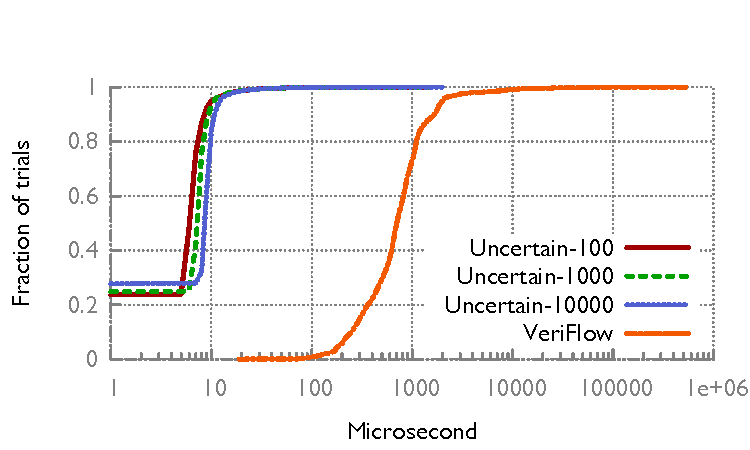
\includegraphics[width=\columnwidth,trim= 0 5mm 0 10mm]{figs/micro}
  \vspace{-0.2in}
  \caption{\em \small Microbenchmark results.}
  \vspace{-0.15in}
  \label{fig:microbench}
\end{figure}

%We observed that 
\name was able to verify 80\% of the updates within 10 $\mu$s, with a 9 $\mu$s mean. 
%In fact, approximately 25\% of the updates were verified within 1 $\mu$s. The reason is that only the minimum change to \name's network model is required for each update, i.e., only one operation in the trie, as indicated by Figure \ref{fig:statemachine}. 
%\wxzc{This sentence (the one refers to fig 8) was used to explain the sentence before it, which is comment off now. So this one needs to be rewritten.}
\name verifies updates almost two order of magnitude faster than VeriFlow because of 
data structure optimizations (\S\ref{sec:impl}). 
Approximately 25\% of the updates were processed within 1 $\mu$s, 
because \name accurately tracks the state of each rule over
time. When a new update matches the pattern of some existing rule, it's likely
only a minimum change to \name's network model is required (e.g., only one
operation in the trie, with no unnecessary verification triggered).
We observed long tails in all curves, but the verification time of \name is bounded by 2.16 ms, almost three orders of magnitude faster than VeriFlow's worst case. 
%which is tolerable for most wide-area network applications. 
%\wxzc{do we need to emphasize ``wide-area" here?}
The results also show strong scalability. As the number of concurrent uncertainty rules grows, the verification time increases slightly (on average, 6.6 $\mu$s, 7.3 $\mu$s, and  8.2 $\mu$s for the 100-, 1000-, and 10000-uncertain-rule cases, respectively). Moreover, \name offers a significant memory overhead reduction relative to VeriFlow: 540 MB vs 9 GB.


%\subsection{Performance Analysis during Network Changes}
\subsection{Performance Analysis}
\label{sec:parallel}

\subsubsection{Emulation-based Evaluation}
%\paragraphb{Emulation-based Evaluation}

\paragraphe{Segment-independent Policies:}
We used Mininet to emulate a fat-tree network with a shortest path routing application and a load-balancing application in a NOX controller. The network consists of five core switches
%\cut{fully connected with} 
and ten edge switches, and each edge switch connects to five hosts. %To initialize the flow table for each switch, each host first picked up a random destination host to perform a file transfer. 
We changed the network (e.g., add links, or migrate hosts) to trigger the controller to update the data plane with a set of new updates. 
%Once the rules were stable in the switches, we changed the network (e.g., add links, or migrate hosts) to trigger the controller to update the data plane with a set of new updates. %We measured the delay that the new rules took to be applied to the network. 
For each set of experiments, we tested six update mechanisms: (1) the controller immediately issues updates to the network, which is \textbf{Optimal} in terms of update speed; (2) \textbf{\name} with the basic connectivity invariant (loop and black-hole freedom) verification enabled (\name); (3) \name with an additional invariant that packets must traverse a specific middle hop before reaching the destination (\name-waypoint); (4) Consistent Updates (\textbf{CU})~\cite{Reitblatt2012}; (5) incremental Consistent Updates (\textbf{Incremental CU})~\cite{incremental-cu}; and (6) \textbf{Dionysus} \cite{jin2014dynamic} with its WCMP forwarding dependency graph generator.
\wxznew{We configure our applications as the same type as in Dionysus, with
forwarding rules matching exactly one flow, i.e., no overlapping forwarding
graphs. Thus, loop and black-hole freedom are segment-independent as proved in
\S\ref{sec:seg-independence}. Because of the fat-tree structure, there is no
crossing between path segments (as in Fig~\ref{fig:circular}(a)), 
so the waypoint policy is also segment independent.}
\wxzcr{A mix of old and new configurations, e.g., 
$oldAB + newBC$ in Figure~\ref{fig:circular}(a), 
is allowed by \name, but forbidden when using CU.}
\wxzcrnew{Note here, we used our implementation of the algorithms introduced in Dionysus paper,
which supports packet coherence.
That is, with extra effort, one can develop algorithms that build customized dependency graphs 
for weaker properties, and thus achieve better efficiency.}

%The CU we used was modified from an implementation developed at Stanford University \cite{standford_cu_imp}. Each experiment was repeated 10 times and we plotted the experimental results in the form of CDF. 

%Here we define {\em controller-switch delay} as the delay between controller issuing an update and the corresponding switch finishing the application of the update. The controller-switch delay is the sum of networking delay (typically on the order of hundreds of microseconds in data center networks), and processing delay (the time a switch takes to apply an update, e.g, installing a flow entry). Flow entry installation speed of commercial SDN switches like Pica8 is around 200 flows per second. 
We first set the delay between the controller issuing an update and the corresponding switch \wxznew{finishing the application of} the update (i.e, the controller-switch delay) to a normal distribution with 4 ms mean and 3 ms jitter, to mimic a dynamic data center network environment. The settings are in line with that of other data center SDN experiments~\cite{curtis2011devoflow, Sherwood10}. We initialized the test with one core switch enabled and added the other four core switches after 10 seconds. The traffic eventually is evenly distributed across all links because of the load balancer application. We measured the completion time of updating each communication path, %, i.e. the completion time of the last update on the path, 
repeated each experiment 10 times.  Figure~\ref{fig:emulation}(a) shows the CDFs for all six scenarios.

The performance of both ``$CCG$" and ``\name-waypoint" is close to optimal, and much faster \kevin{(47 ms reduction on average)} than CU. %To avoid the rare situations of infeasible update orderings with pure \name (though we did not encounter any in this set of experiments), we integrated the \name with CU to ensure the same consistency level (e.g., absence of black holes and loops). 
%``\name+CU" is 15 ms slower than \name alone in average because of the additional cost of packet transformation, versioning, and rule classification, but it is still 20 ms faster in average than CU. 
%It is because CU holds the network invariants by ensuring that all packets can only be handled by either the old rules or the new rules via a two-phase update mechanism. 
In CU, the controller is required to wait for the maximum controller-switch delay to guarantee that all packets can only be handled by either the old or the new rules. 
%across all the switches, before proceeding to phase two to complete the update. 
\name relaxes the constraints by allowing a packet being handled by a mixture of old and new rules along the paths, as long as the impact of the new rules passed verification. By doing so, \name can apply any verified updates without explicitly waiting for irrelevant updates. 
%In addition, \name can aggregate more updates to individual network devices. CU or incremental-CU, on the other hand, have to distinguish {\em edge rules} and {\em internal rules} and apply them in separate phases. \wxzc{not sure it's necessary to mention the benefit of aggregation?} 
%The memory usages for all five scenarios are presented in \fixme{Figure X}. 
CU requires temporary doubling of the FIB space for each update, %Many SDN switches use TCAM memory, which is both expensive and power-consuming. It is because in CU, packets handled by each configuration are tagged with different version numbers to avoid encountering a mix of configurations. 
because it does not delete old rules until all in-flight packets processed by the old configuration have drained out of the network. To address this, incremental-CU was proposed to trade time against flow table space. By breaking a batch of updates into $k$ subgroups ($k=3$ in our tests), incremental-CU reduced the extra memory usage to roughly one $k$th at the cost of multiplying the update time $k$ times. %but took much longer to apply all updates ($k$ times of the delay using CU). 
\wxznew{In contrast, when dealing with segment-independent policies, as in this set of experiments,} \name never needs to trigger any heavyweight fallback plug-in, and thus requires no additional memory, which is particularly useful as switch TCAM memory can be expensive and power-hungry.

%Also, \name reduces the expensive packet modifications that are required by the CU design to enforce versioning. We also observed in Figure~\ref{fig:emulation}(a) that the verification process only adds a little overhead to the update completion time as compared with the optimal case. 

%The second set of experiments evaluated the system update delay with dynamic host settings. We used all five core switches and ten edges switches throughout the experiments. Initially, each host sent traffic to another randomly selected host. After 10 seconds, we randomly re-distributed 40\% of the connections between hosts and edge switches, and then started the file transfer again. The results are in Figure~\ref{fig:emulation}(b). We observed that the gap between \name and the optimal case is larger (around 30 ms) than the results in the first set of experiments. It is because host position changes resulted in almost a complete change of the relevant paths, and thus complicates the inter-dependency among the new rules. But still \name outperformed CU by 20 ms per update on average. 

\begin{figure}[!th]
  \centering
  \vspace{-0.1in}
  \subfigure[Data center network setting]{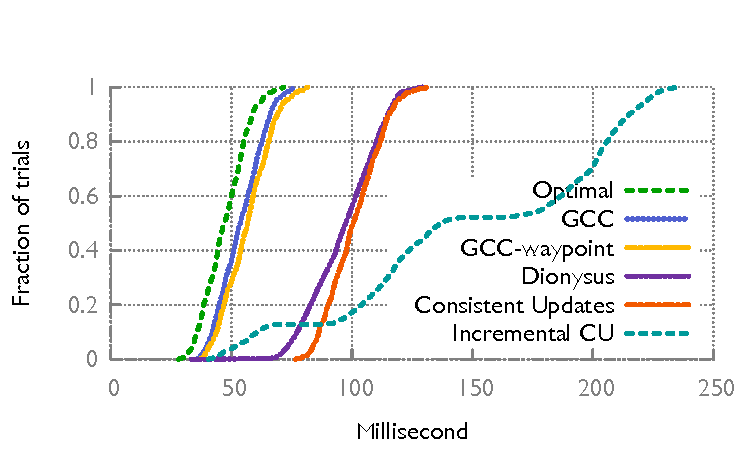
\includegraphics[scale=0.6,trim=0mm 0mm 0mm 10mm]{figs/emulation_4ms}}%
  \vspace{-0.1in}
  %\subfigure[Data Center Network, Transition with Host Migration]{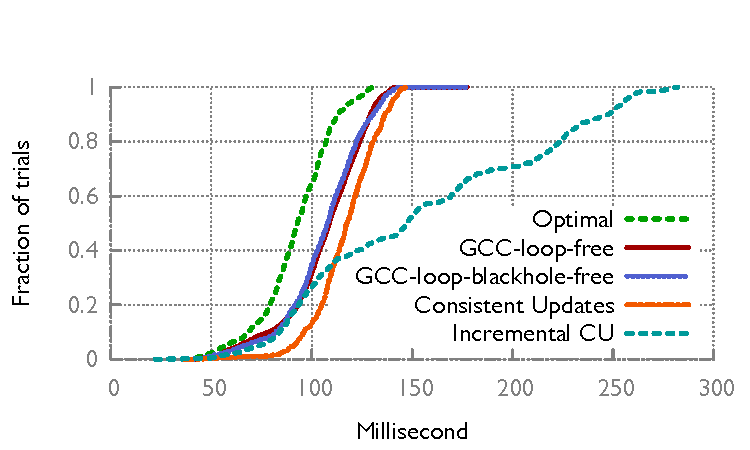
\includegraphics[scale=0.6,trim=0mm 0mm 0mm 1mm]{figs/emulation_dynamic_1ms}}
  \subfigure[Wide-area network setting]{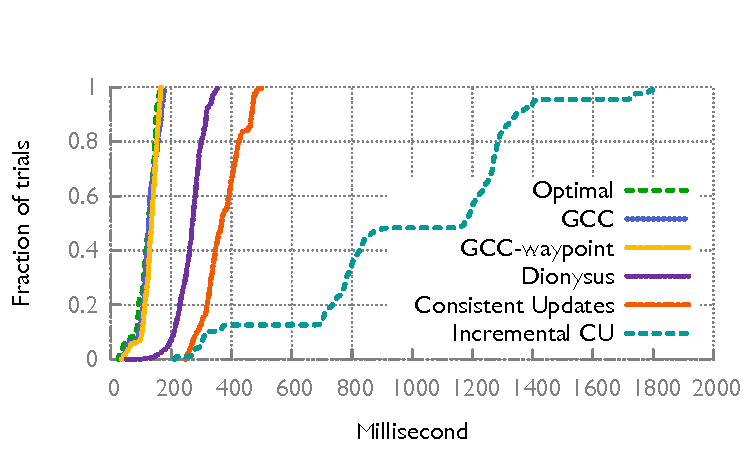
\includegraphics[scale=0.6,trim=0mm 0mm 0mm 1mm]{figs/emulation_100ms}}
  %\subfigure[Wide-area Network, Transition with Host Migration]{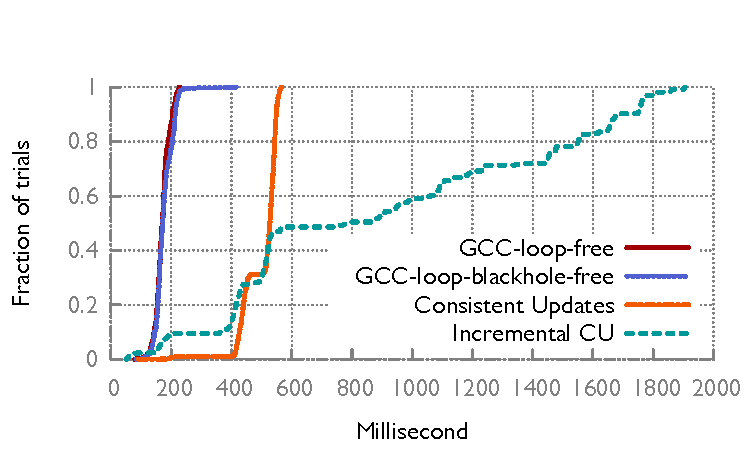
\includegraphics[scale=0.6,trim=0mm 0mm 0mm 1mm]{figs/emulation_dynamic_25ms}}
  %\vspace{10pt}
  \vspace{-0.1in}
  \caption{\em \small Emulation results: update completion time comparison.}
  \vspace{-0.3in}
  \label{fig:emulation}
\end{figure}

To understand how \name performs in wide-area networks, 
where SDNs have also been used~\cite{jain2013b4, Hong13}, 
we set the controller-switch delay to 100 ms (normal distribution, 
with 25ms jitter), and repeated the same tests (Figure \ref{fig:emulation}(b)). 
\name saved over 200 ms update completion time compared to CU,  mainly due to the longer controller-switch delay, for which CU and incremental-CU have to wait between the two phases of updates. %Besides the network changes with link addition, we also experiment the systems with dynamic host migration, and observed the similar performance gain of \name as compared with CU and ICU. 

\wxznew{
As for Dionysus, 
we observed in Figure~\ref{fig:emulation}
that it speeds up updates compared to CU in both local and wide-area
settings, as it reacts to network dynamics rather than \pbg{pre-determining} a
schedule. But because its default algorithm for WCMP forwarding produces
basically the same number of updates as CU, 
\name (either \name or \name-waypoint)
outperforms it in both time and memory cost.
We further compared \name-waypoint with Dionysus in other dynamic situations, 
by varying controller-switch delay distribution.
Figure~\ref{fig:dn} shows the $50^{th}$, $90^{th}$ and $99^{th}$ percentile 
update completion time, under various controller-switch delays
(normal distributed with different (mean, jitter) pairs, $(a, b)$) for 
four update mechanisms: optimal, \name, Dionysus, and CU. 
In most cases, both \name and Dionysus 
outperform CU, with one exception (4ms delay, zero jitter).
Here, Dionysus does not outperform CU because
it adjusts its schedule according to network dynamics, 
which was almost absent in this scenario.
The cost of \wxzcrnew{updating} dependency graphs in this scenario
is relatively large compared to the small network delay. \fixme{you are including compute time in the evaluation?  That's OK, but explain it}
When the mean delay was larger (100ms), even with no jitter,
Dionysus managed to speed the transition by updating each forwarding path independently.}
On the other hand, \name's performance is closer to \pbg{Optimal} than Dionysus. For example, in the $(4, 0)$ case,  \name is 37\%, 38\%, and 52\% faster than Dionysus in the $50^{th}$, $90^{th}$ and $99^{th}$ percentile, respectively; in the $(100, 25)$ case,  \name is 50\%, 50\%, and 53\% faster than Dionysus in the $50^{th}$, $90^{th}$ and $99^{th}$ percentile, respectively. Also, we observe that Dionysus's performance is highly dependent on the variance of the controller-switch delay (the larger the jitter is, the faster the update speed) because of the dynamic scheduling, but \name's performance is insensitive to the jitter.

\begin{figure}[!ht]
  \centering
  \vspace{-0.1in}
  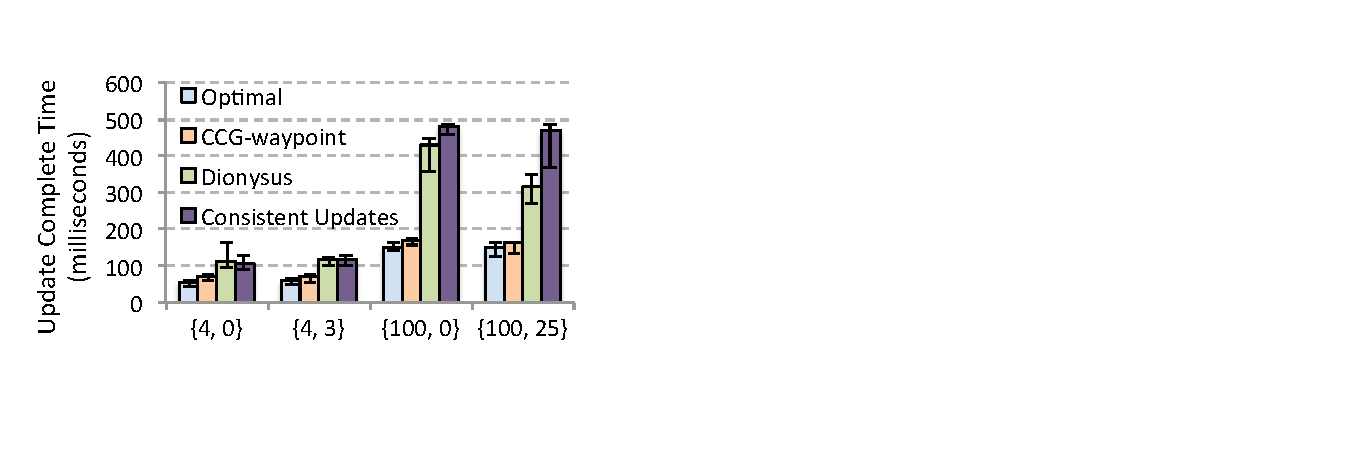
\includegraphics[width=0.8\columnwidth]{figs/distribution_narrow.pdf}
  \vspace{-0.1in}
  \caption{\em Update completion time with [$50^{th}$, $90^{th}$, $99^{th}$ percentile]; x-axis label \{a, b\}: a is the mean controller-switch delay, b is the jitter following a normal distribution.}
  \vspace{-0.2in}
  \label{fig:dn}
\end{figure}

\paragraphe{Non-segment-independent Policies:}
\kevin{
We then explored scenarios in which \name's lightweight heuristic cannot always synthesize a correct update ordering and needs to fall back to the more heavyweight algorithm to guarantee consistency. The traces we used were collected from a relatively large enterprise network that consists of over 200 layer-3 devices.
%\cut{Each device has around 13,000 to 15,000 rules in average.}
\wxznew{During a one-day period (from 16:00 7/22/2014 to 16:00 7/23/2014), we took one snapshot of the network per hour, and used Mininet to emulate 24 
transitions, each between two successive snapshots.}
%\cut{The data covers the duration of one day (from 16:00 7/22/2014 to 16:00
%7/23/2014), and was divided into 24 one-hour windows. For each window, we
%took a new snapshot of the network states, and performed a transition from
%the previous snapshot to the current one. }
We processed the network updates
with three mechanisms: immediate application of updates, \name, and CU.
\wxzcr{Updates were issued such that new rules were added first, then old rules deleted.
Thus, all three mechanisms experience the trend that the number of stored rules increases
then decreases.}.
The controller-switch delay was set to 4 ms. We selected 10 strongly
connected devices in the network, and plotted the number of rules 
in the network over time during four transition windows, as shown in
Figure \ref{fig:cise}. As the collected rules overlapped with longest prefix match,
the resulting forwarding graphs might share links, so unlike previous experiments,
segment-independency was not guaranteed.

%We observed 
The update completion time (\wxznew{indicated by the width of
the span of each curve}) using \name was much shorter
%(around x\% shorter on average with the standard deviation y\%) 
than CU, and the memory
needed to store the rules was much smaller.
%(around x\% smaller on average, with the standard deviation y\%). 
In fact, the speed and memory requirements of \name 
were close to those of the immediate update case, because
\name rarely needs to fall back to CU. In 22 out of 24
windows, there was a relatively small number of network updates (around 100+),
much as in the [22:00, 23:00) window shown in Figure \ref{fig:cise},
%\wxzc{This window is an example of one of the windows}
in which \name
passed through most of the updates with very few fallbacks. During the period 23:00
to 1:00, there was a burst of network dynamics (likely to have been 
caused by network maintenance), in which 8000+ network
updates occurred. Even for such a large number of updates, the
number of updates forced to a fallback to CU, was still quite small (10+).
\wxzcr{Since \name only schedules updates in a heuristic way,
the waiting time of a buffered update could be suboptimal, as in this hour's case,
where the final completion time of \name was closer to CU.}
%\cut{In addition, even for the fall back scenarios, the
%rules that triggers the fallbacks are actually a subset of the entire rules
%required by CU, which essentially} 
%Thus we can see, \name significantly reduces the
%memory requirement and increases the processing speed. On the other hand,
\name achieves performance comparable to the immediate update mechanism, but without
any of its short-term network faults (24 errors in the 0:00 to 2:00 period).

%With performance typically comparable to the immediate update mechanism,
%(the ideal case in terms of speed and memory), 
%\name did not suffer from any short-term
%network fault as the immediate update did
%\cut{due to inconsistence updates} 
%(e.g., 24 errors in the 0:00 to 2:00 period). 
%This demonstrates \name's ability to achieve nearly the
%``best of both worlds": the efficiency of passing through updates in
%most cases, with the consistency guarantees of more heavyweight solutions.  
}

%handle packet transformation
%during fall back, also handle packet transformation
%this time, prefix matching -> one rule affect multiple forward graphs. the orders from graph maybe conflict
%in fat tree topo + exact matching

\begin{figure*}[!ht]
  \vspace{-0.1in}
  \centering
  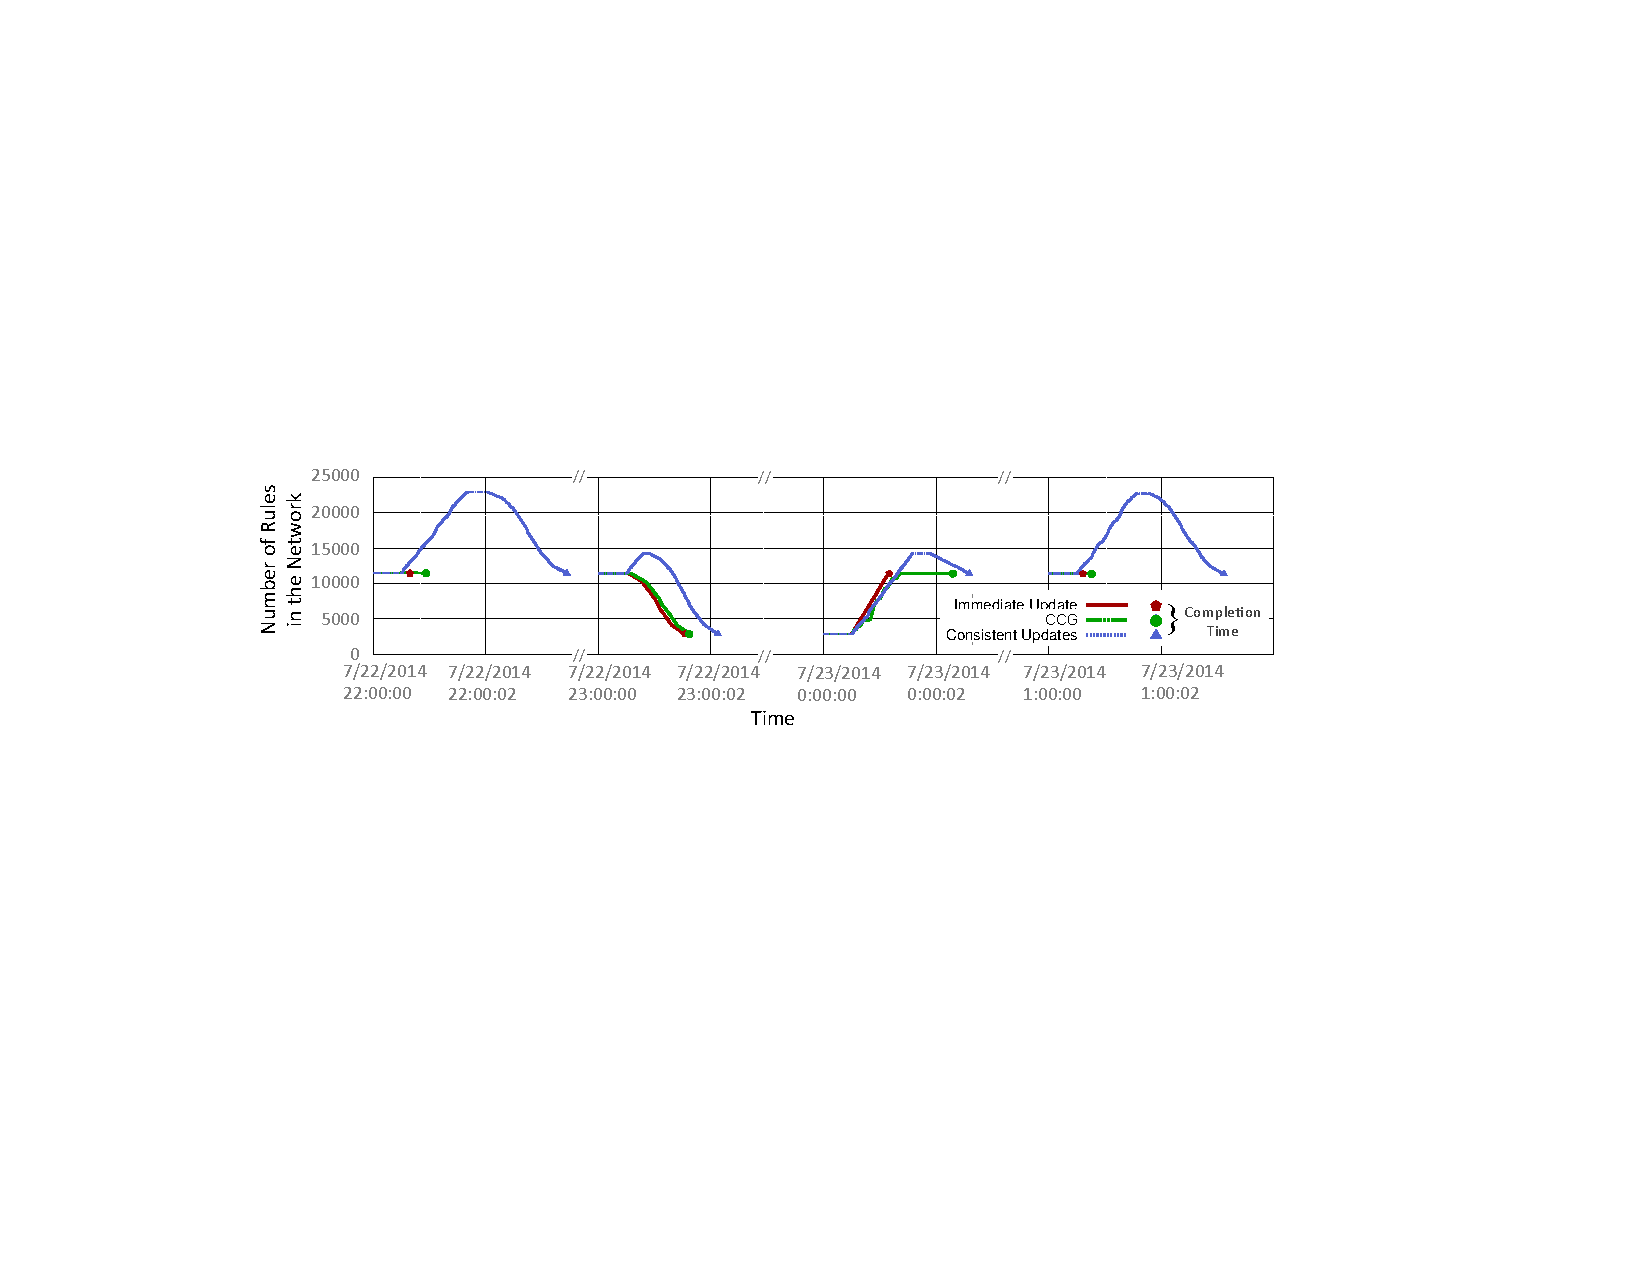
\includegraphics[width=0.9\textwidth]{figs/count.pdf}
  \vspace{-0.15in}
  \caption{\em Network-trace-driven emulations: (1) immediate application of updates; (2) \name (with CU as fallback); and (3) CU.}
  \vspace{-0.2in}
  \label{fig:cise}
\end{figure*}


\subsubsection{Physical-testbed-based Evaluation}
%To test real world distributed timing effects, 
%\paragraphe{Physical-testbed-based Evaluation:}
We also evaluated \name on a physical SDN testbed~\cite{ocean}
consisting of 176 server ports and 676 switch ports, using Pica8 Pronto 3290 switches via TAM Networks, NIAGARA 32066 NICs from Interface Masters, and servers from Dell.
We compared the performance of \name and CU by monitoring the traffic
throughput during network transitions. We first created a network
with two sender-receiver pairs transmitting TCP traffic on gigabit links, 
shown in Figure \ref{fig:s_topo}. Initially, a single link was shared by the
pairs, and two flows competed for bandwidth.  After 90 seconds, another path
was added %\cut{for one of the pairs}
(the upper portion with dashed lines in
Figure \ref{fig:s_topo}). Eventually, one flow was migrated to
the new path and each link was saturated. 
% We are interested to explore the system behaviors during the network changes. 
We repeated the experiment 10 times, and recorded the average throughput in a 100-ms window during the network changes. We observed repeatable results.  Figure~\ref{fig:testbed}(a) shows the aggregated
throughput over time for one trial.

\name took 0.3 seconds less to finish the transition than CU because: (1) unlike CU, \name does not require packet modification to support versioning, which takes on the order of microseconds for gigabit links, while packet forwarding is on the order of nanoseconds; (2) CU requires more rule updates and storage than \name, and the speed of rule installation is around 200 flows per second; and (3) Pica8 OpenFlow switches (with firmware 1.6) cannot simultaneously process rule installations and packets.\footnote{All the performance specifications reported in this paper have been confirmed with the Pica8 technical team.} %We also noticed that, besides delayed network transition, the amount of the extra work required by CU also resulted in some temporary throughput drops (as shown in Figure \ref{fig:testbed}(a)). 
%because of the long rule processing and buffering time. 
%However, such drops did not occur in \name throughout all of our experiments.

\begin{figure}[!ht]
  \centering
  \vspace{-0.1in}
  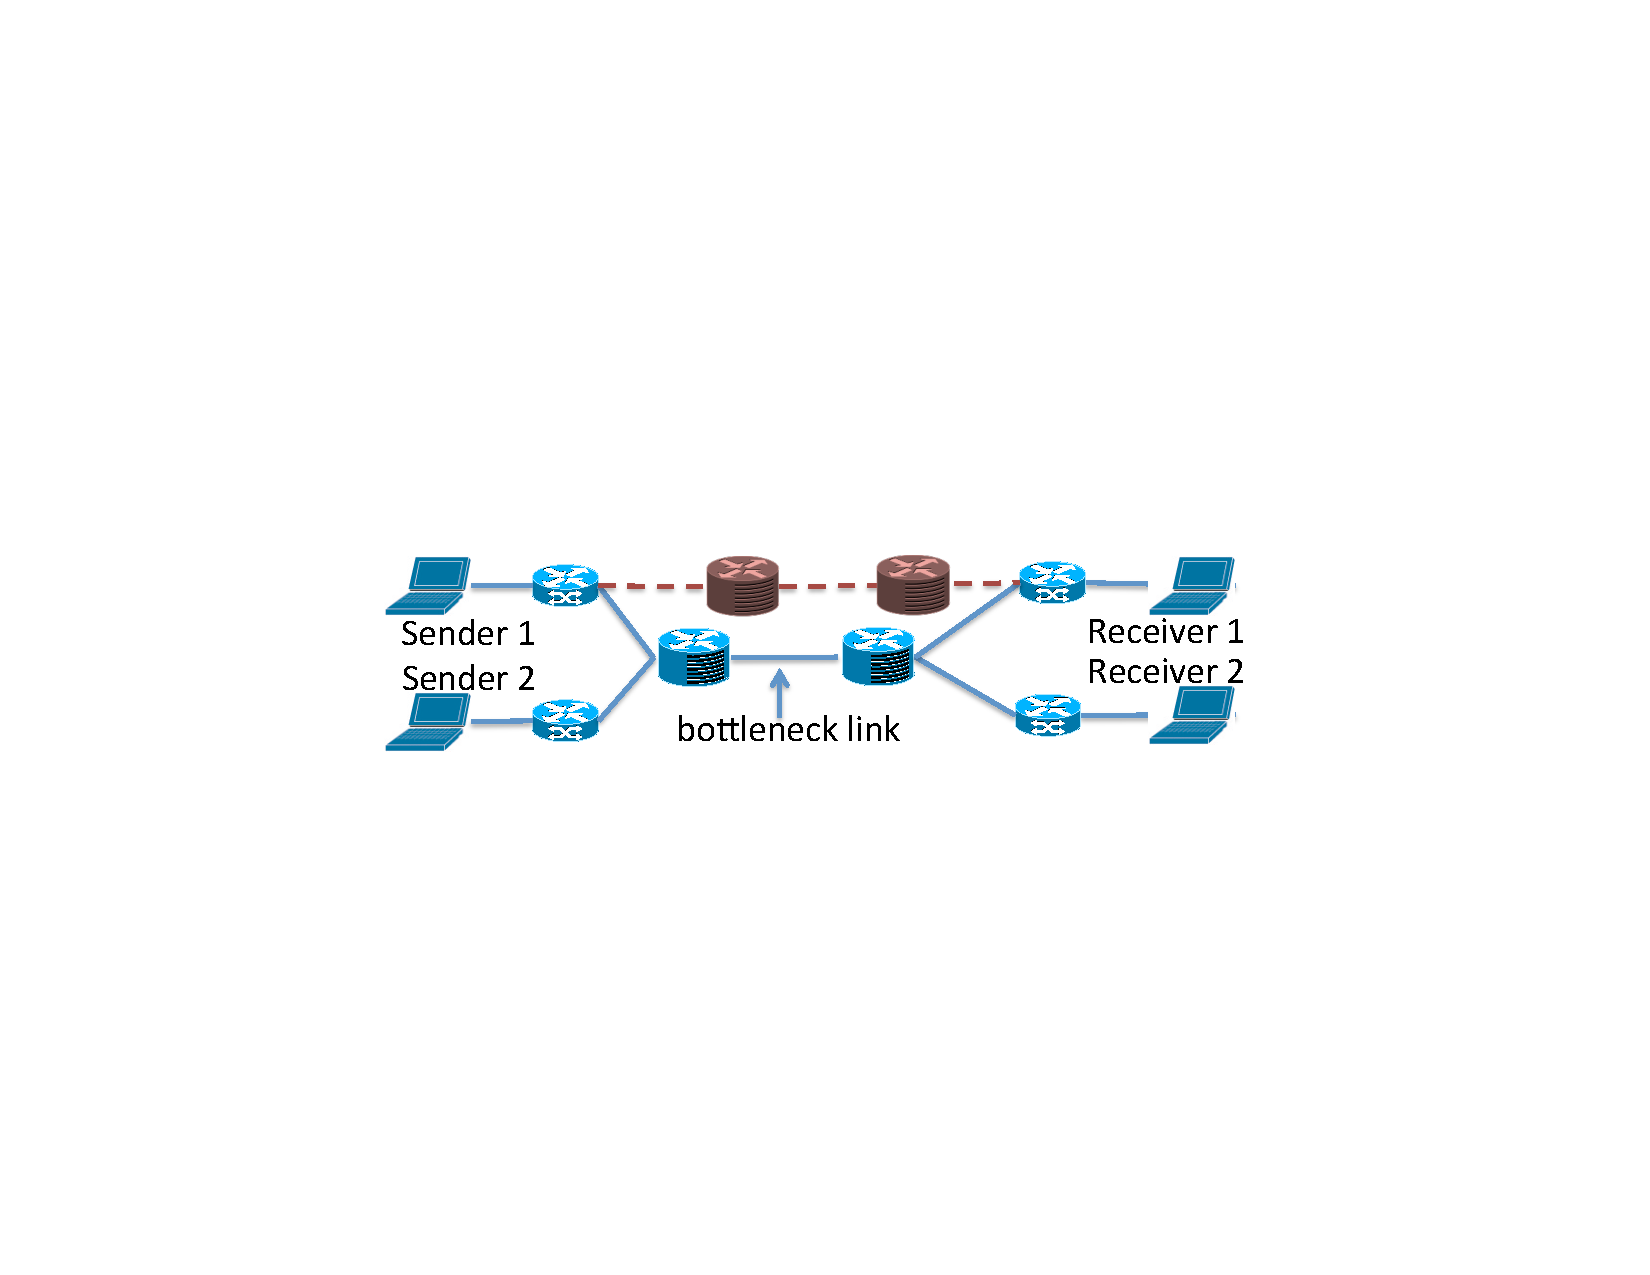
\includegraphics[width=0.7\columnwidth]{figs/dumbell_topo}
  \vspace{-0.1in}
  \caption{\em eight-switch topology.}
  \vspace{-0.15in}
  \label{fig:s_topo}
\end{figure}

\begin{figure}[!ht]
  \centering
  \vspace{-0.1in}
  \subfigure[A eight-switch topology.]{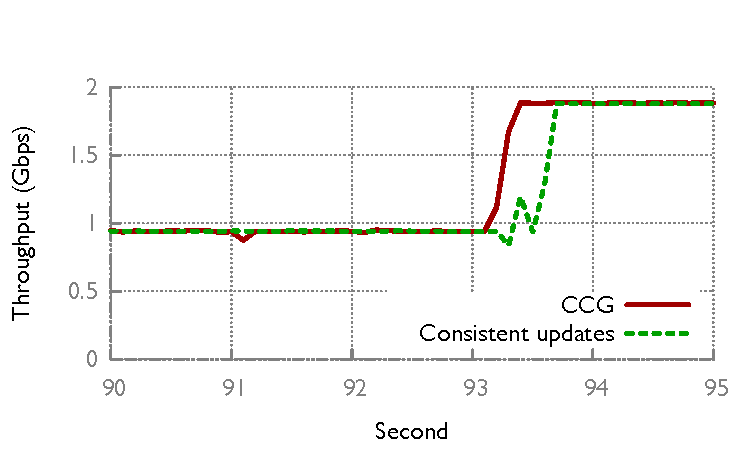
\includegraphics[width=0.8\columnwidth,trim=0mm 0mm 0mm 12mm]{figs/testbed_subspace_small}}%
  \vspace{-0.1in}
  %\subfigure[Throughput Changes during Network Transitions on a Small-scale Network with 6 Switches]{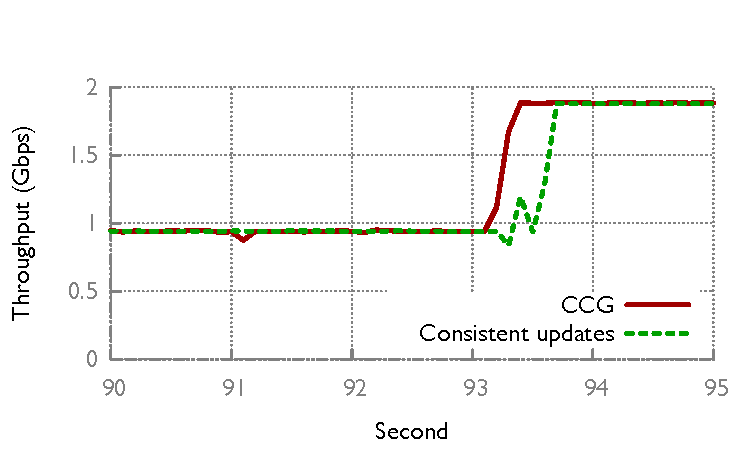
\includegraphics[width=\columnwidth,trim=0mm 0mm 0mm 12mm]{figs/testbed_subspace_small}}
  \subfigure[A 78-switch network.]{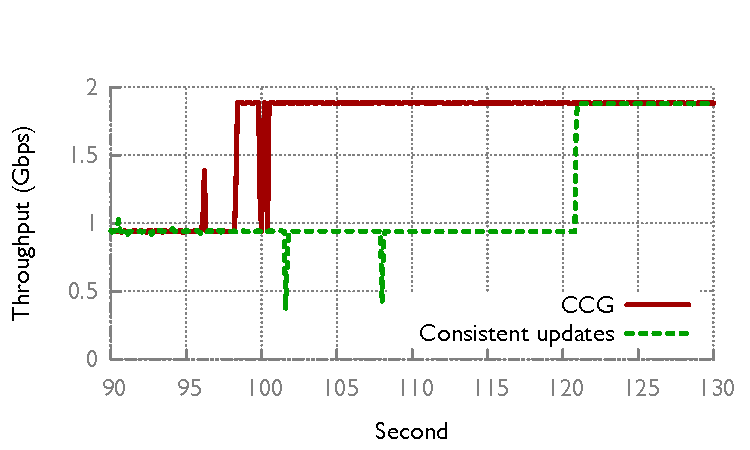
\includegraphics[width=0.8\columnwidth,trim=0mm 0mm 0mm 2mm]{figs/testbed_full}}
  \vspace{-0.1in}
  \caption{\em \small Physical testbed results: comparison of throughput changes during network transitions for \name and CU.}
  \vspace{-0.3in}
  \label{fig:testbed}
\end{figure}

%\if 0
%We created a biggest fat tree topology with X core switches and Y edge switches by slicing the 13 physical SDN switches. The virtual topology to physical topology mapping algorithm was developed using the GUROBI optimization package \cite{gurobi}. We are using same NOX controller applications as we used for the emulation experiments. Initially, we set the flow tables of the switches to enable only N core switches, and all hosts sent traffic to every other host for 10 seconds. We then alter the switch flow tables to bring in all the remaining core switches, and more flows would be migrated to the new core switches for load balancing. We measure the throughput and the flow drop rate for the CU, incremental CU, and \name for comparison. The results are shown in Figure \ref{fig:testbed}. [to change]
%\fi
\wxzcr{To test \name in a larger setting, 
%we then created a topology utilizing all 13 physical SDN switches. 
we then utilized all 13 physical switches. 
Each physical switch was devided into 6 ``virtual" switches by creating 6 bridges.
Due to the fact that the switches are physically randomly connected,
this division results in a ``pseudo-random" network consisting of 78 switches, each with 8 ports.} 
%Eight ports were attached to each virtual switch and the port assignment was computed with our mapping algorithm, which was developed using the GUROBI optimization package \cite{gurobi}. The mapping algorithm ensures that each attached virtual host had at least one path to every other host, subject to the physical cabling. 
Initially, the topology consisted of 60 switches, %and each switch was connected to two hosts. 
and we randomly selected 10 sender-receiver pairs to transmit TCP traffic. %, and each sender and the corresponding receiver were attached to different virtual switches. 
After 90 seconds, we enabled the remaining 18 switches in the network. 
The topology change triggered installations of new rules to balance load. % under the command of the NOX controller. 
We repeated the experiments 10 times, 
%and measured throughput of each flow. We 
and selected two flows from one trial that experienced throughput changes
%, and show the changes over time in a 100 ms window 
(Figure~\ref{fig:testbed}(b)). The trend of the two flows is consistent with the overall observed throughput change. %The selection criteria of the two flows are that they shared common links before the transition and used two disjoint paths after the transition, and there was no cross-traffic from other flows on their paths. %This way, comparison with the results in the first set of experiments under larger network state changes is straigtforward. The results are shown in Figure \ref{fig:testbed}(b). 

%We observed a similar trend as in the small topology setting; 
\name again outperformed CU in convergence time and average throughput during transitions. Compared to CU, \name spent 20 fewer seconds to complete the transition (a reduction of 2/3), because CU waits for confirmation of all updates in the first phase before proceeding to the second.
%, and the performance drops dramatically as the number of updates increases. 
In contrast, \name's algorithm significantly shortened the delay, especially for networks experiencing a large number of state changes. In \name, the throughput never dropped below 0.9 Gb/s, while CU experienced temporary yet significant drops during the transition, primarily due to the switches' lack of support for simultaneous application of updates and processing of packets. %\wxznew{We are still researching on the explanation, and one possible reason is switches' lack of support to parallelize operations.}


\if 0
\subsection{Network Fault Detection Coverage}
\label{sec:bug-coverage}

Failing to consider the temporal uncertainty of the network may result in transient or permanent network faults that can affect security and performance. In this set of experiments, we explore how \name can help to improve the error detection coverage by modeling network uncertainty. We used the same network topology consisting of that we used for the speed analysis in \S~\ref{sec:microbenchmark}. We replayed 2,559,251 BGP FIB changes into \name and VeriFlow, and verified the network against forwarding loops and blackholes using both systems. Results are shown in Table~\ref{tab:bug_coverage}. 

\begin{table}
\footnotesize
\caption{Error Coverage Comparison: VeriFlow vs \name}
\label{tab:bug_coverage}
\begin{tabular}{|p{1.8cm}|p{2.1cm}|p{1.5cm}|p{1.7cm}|}
%\begin{tabular}{|l|c|c|}
\hline
Error Type & Found by Veri- & Only \name   & Only \name \\
& Flow \& \name & (Potential) & (Certain)\\
\hline \hline
Black Hole &1,037,866 & 362,460 & 125,808 \\ \hline
Loop & 28,936 &166,508 & 166,991 \\ \hline
Out of Order Updates & N.A. & 362,408 & N.A. \\ \hline
Total & 1,066,802 & 891,376 & 292,799 \\ \hline
\end{tabular}
\end{table}

The second column shows the number of errors that are detected by both VeriFlow and \name. 
We measure three types of errors: black holes, loops, and out of order updates -- the last of which refers to updates that trigger a race condition on switches, e.g., addition and withdrawal of the same rule without a barrier between them. 
We found that \name does not miss any errors that VeriFlow captures. The third and fourth column show the number of  errors that \name is able to capture, but are missed by VeriFlow, among which 891,376 errors are reported by \name's verification engine as errors that may exist, and 292,799 as certain errors. 
\fi
% The errors are categorized into three types, black hole, loop, and out of order updates.
%For loops, although the algorithm for computing BGP updates should produce loop-free solutions,
% (which is why VeriFlow did not report any loop), transient loops did exist in the network because of the uncertain timing and ordering of the update installations. 
%The additional black holes caught by \name include cases where the controller attempted to install an update before all the downstream rules applied. 
%%Out of order updates refers to an error caused by the inconsistency between the order that an controller issues the updates of a switch and the order that the switch actually applies the updates. 
%Out of order updates were caused by updates that trigger a race condition on switches, e.g., addition and withdrawal of the same rule without a barrier between them. 
%%The root cause is the indeterministic update installation behaviors at the switches.
%Note that there is no confirmed out of order updates errors, because our network model will enter the ``unknown" state in this case as explained in the previous section (Figure~\ref{fig:statemachine} in \S~\ref{sec:impl}). VeriFlow did not report those errors by assuming that an update takes effect immediately, but \name is able to capture those errors with the build-in uncertainty-aware network model.
%
%\if 0
%Our system is capable to report many more potential transient errors during network changes than VeriFlow does. One nature question to ask is that if the significant increment on the number of detected errors will have great negative impact on system performance? The experiments results in Section \ref{sec:microbenchmark} show small cost of verification (delay in the order of microsecond). Even if the network scenario is very sensitive to the network latency, it is flexible to tune our system to block rules which results in the occurred errors and apply rules only causing the potential errors.
%\fi
%
%
%\if 0
%Our system have the ability to report many potential transient errors during network changes. It is true that some errors are more important than others, and even the same type of errors can have different impact on different system. For example, loops and black holes which causes temporary long end-to-end delay are not be tolerable in real-time industrial control networks, while such short-term delays is not that important for P2P file sharing networks. \name is currently designed to report all potential transient errors, since we do not want miss the important ones. We will leave the prioritization and classification of the errors as our future work.
%\fi
%

%Limitations: false positive
